% !TEX root = ./main.tex




% Add additional cases by creating a "case_name.tex" file with a corresponding "figures_name" directory to hold all of your figures for that case. This will help keep organized and avoid conflicts. Lastly, simply add an include statement lie those above for your new case. Don't forget to "git add" and commit/push your changes up to the master.

% Flat plate
% !TEX root = ./main.tex
\graphicspath{{figures_flatplate/}}% Set graphics path location

\subsection{Subsonic laminar flat-plate}

Computations of the flow over a subsonic flat-plate have been performed and validated against the Blasius' solution for laminar boundary layer. The flow conditions are Mach number $0.5$, angle of attack $0.0\deg$ and Reynolds number based on the plate length of $1\cdot10^6$. The governing equations are the 2D Navier-Stokes equations with constant ratio of specific heats of $1.4$, Prandtl number of $0.72$ and constant dynamic viscosity of $1.827\cdot 10^{-5} Pa \cdot s$.

\begin{center} 
    \begin{tabular}{l*{5}{c}r}
    Height first cell \& \# of cells inside the boundary layer & Poly order 3 & Poly order 4 & Poly order 5 & Poly order 6 \\ \hline
    Mesh a0 (140 = 14x10). 0.00075 / 2 cells & $\times$ & $\times$ & $\times$ & \Checkmark \\ \hline
    Mesh a1 (560 = 28x20). 0.000375 / 4 cells &  $\times$ & $\times$ & \Checkmark & \Checkmark \\ \hline
    Mesh a2 (2240 = 56x40). 0.0001875  / 8 cells & $\times$ & \Checkmark & \Checkmark & \Checkmark \\ \hline
    Mesh a3 (8960 = 112x80). 0.0000935  / 16 cells & \Checkmark & \Checkmark & \Checkmark & \Checkmark \\
    \hline
    \end{tabular} 
      \captionof{table}{HiFiLES convergence using different grids and polynomial order} \label{table:convergence} 
\end{center}

The objective of this study is to determine the minimum number of elements and the order of polynomial required to converge the flat-plate simulation using HiFILES. In particular, 4 different numerical grids have been used in this study (2, 4, 8, 16 elements inside the boundary layer). The results are summarized in Table \ref{table:convergence}, the simulations require a minimum number of elements in the boundary layer to obtain a satisfactory converge, otherwise, there will be noticeable jumps across the elements.

\begin{figure}
\begin{center}
\begin{minipage}[t]{0.48\columnwidth}
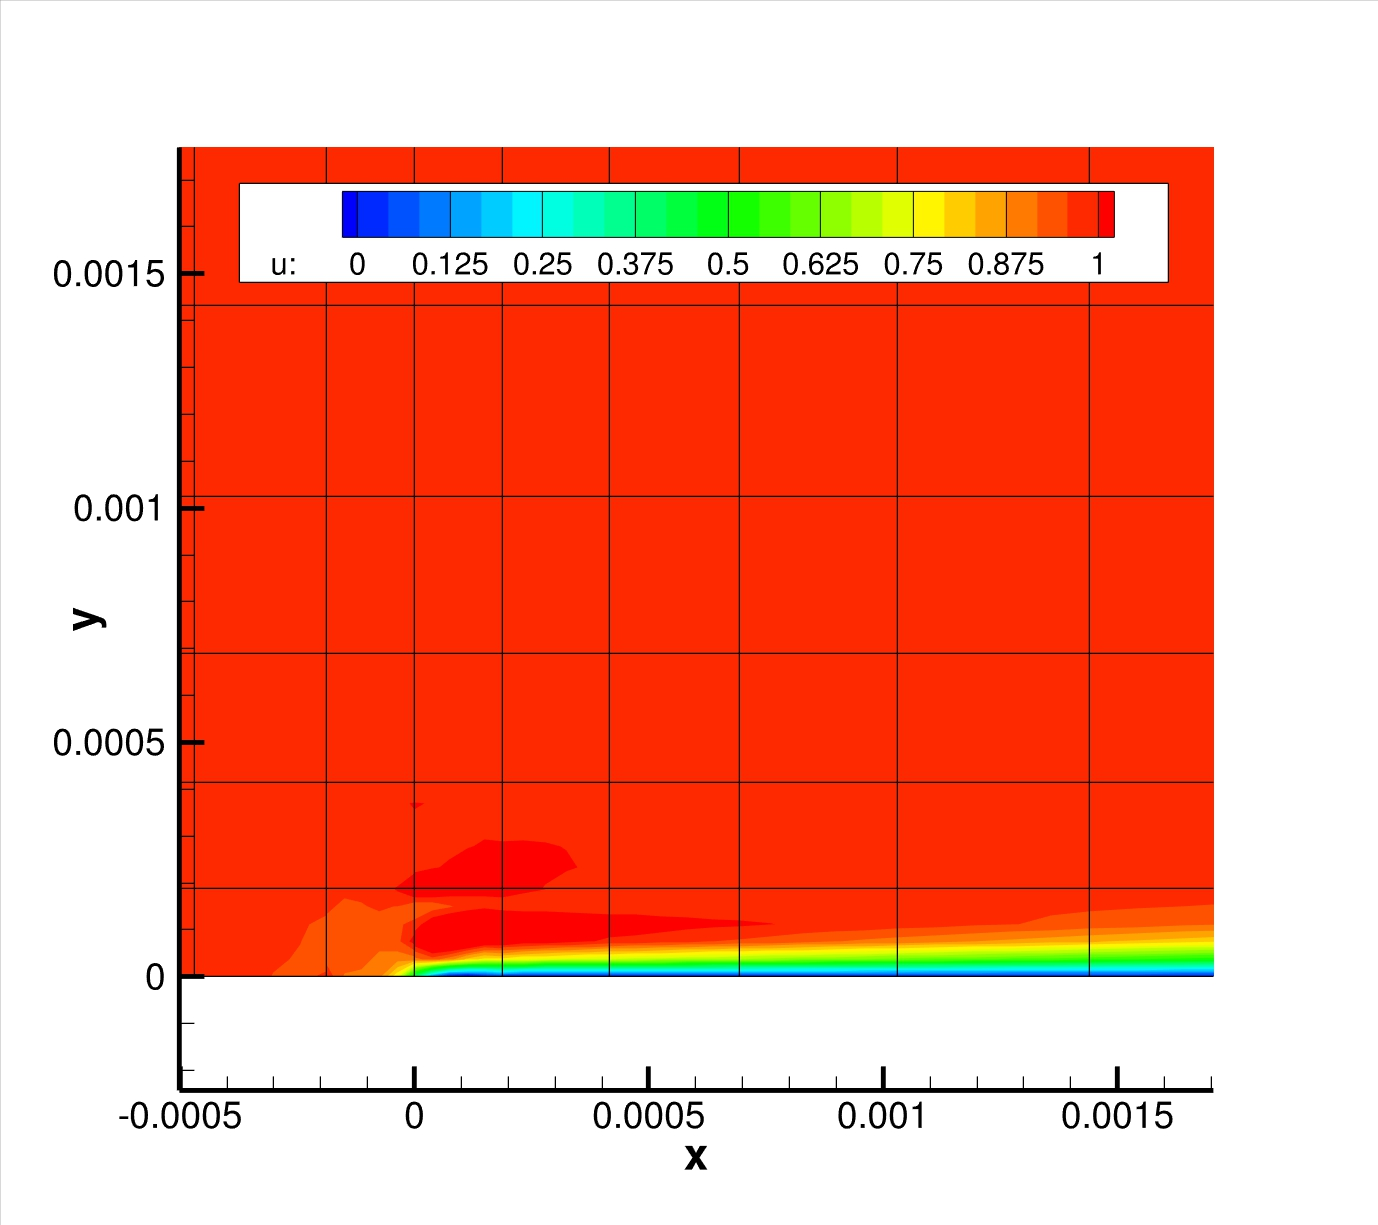
\includegraphics[width = \textwidth,clip=]{LeadingEdge.jpg}
\caption{Detail of the flat-plate leading edge (x=0.0, mesh a2).}
\label{fig:LeagingEdge}
\end{minipage}
\hfill
\begin{minipage}[t]{0.48\columnwidth}
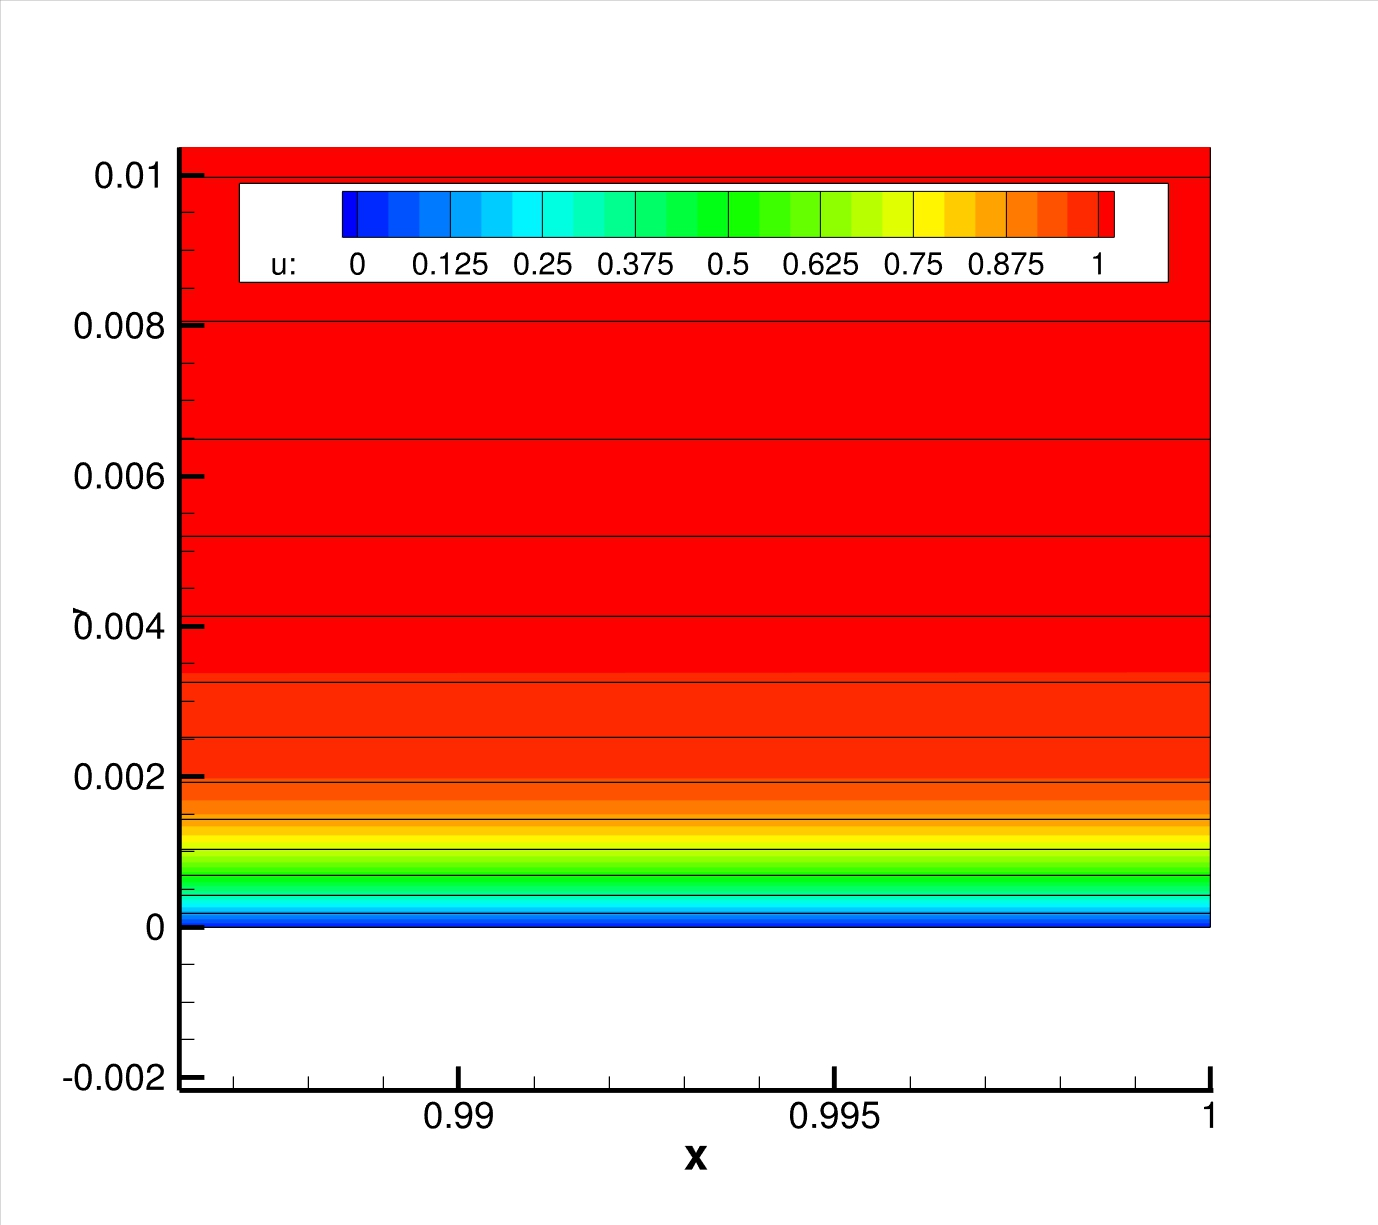
\includegraphics[width = \textwidth,clip=] {EndPlate.jpg}
\caption{Flow solution at the end of the flat-plate (x=1.0, mesh a2).}
\label{fig:TrailingEdge}
\end{minipage}
\end{center}
\end{figure}

The results has been compared with the Blasius' solution for laminar boundary layer with satisfactory results, and some details of the solutions are presented in Fig. \ref{fig:LeagingEdge} (leading edge), and Fig. \ref{fig:TrailingEdge} (end of the flat-plate). It is important to note that in this particular case (mesh a2) the flap-plate is captured using 8 elements, while in a second order solver it would be necessary of the order of ~30 elements inside the boundary layer.

\begin{figure}
\begin{center}
\begin{minipage}[t]{0.48\columnwidth}
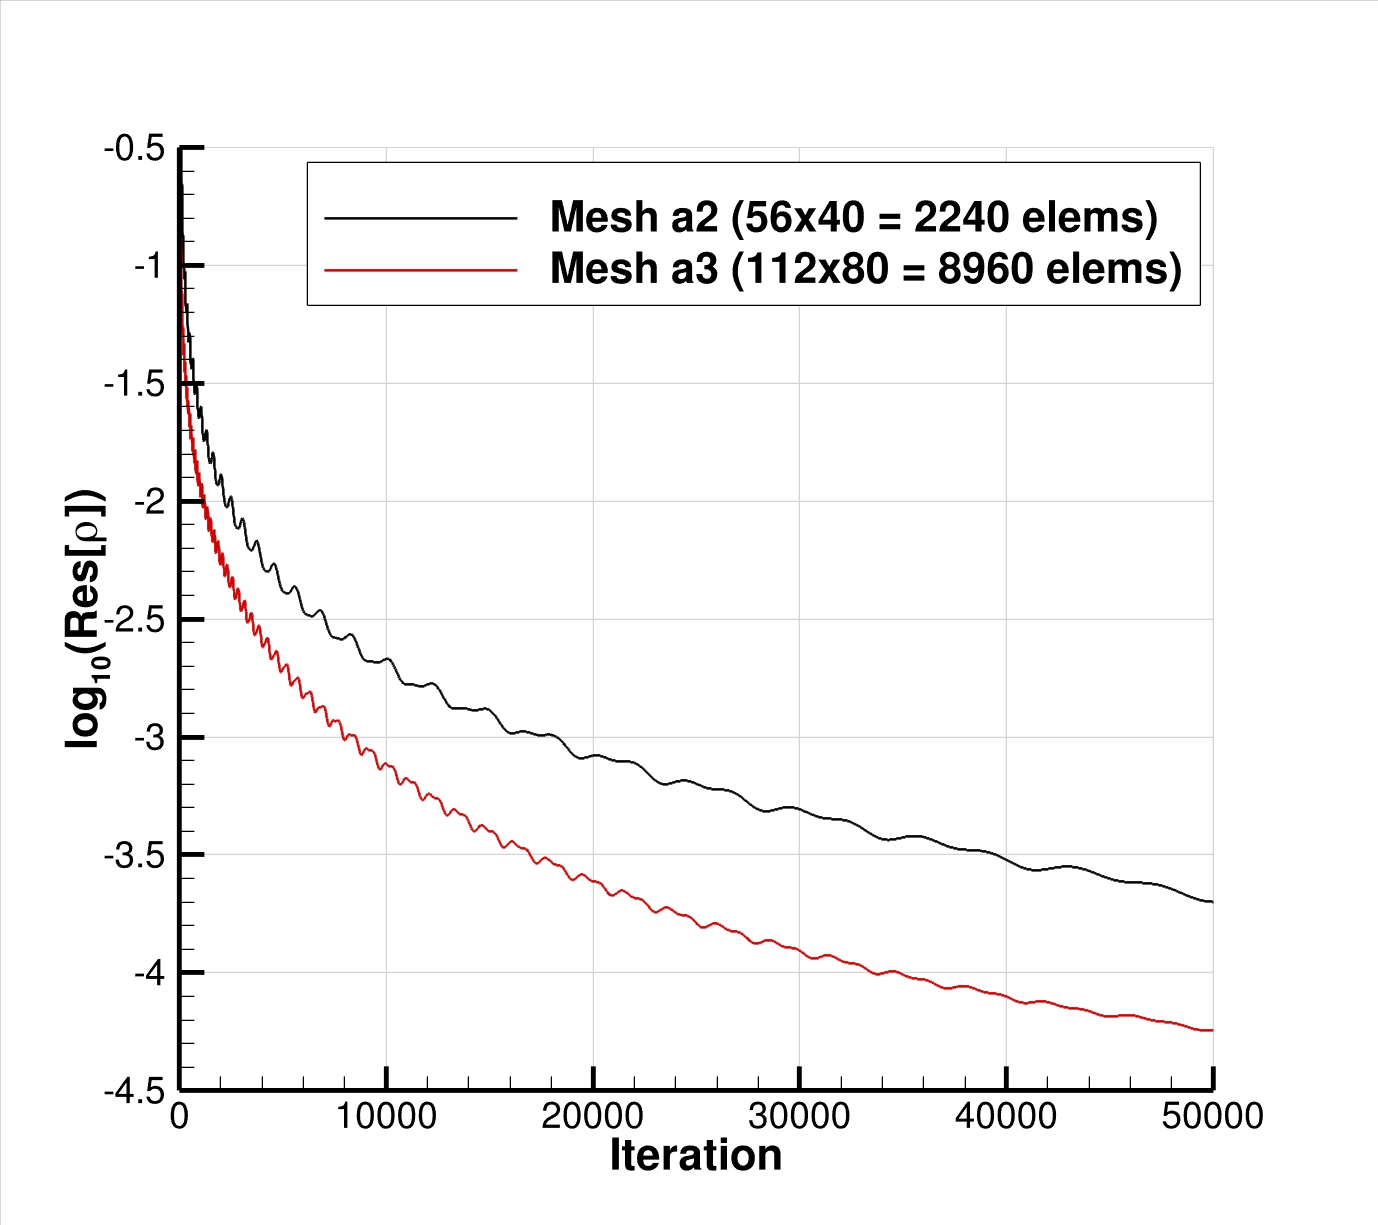
\includegraphics[width = \textwidth,clip=]{CompMesh.jpg}
\caption{Convergence comparison (3$^rd$ order, finest grids).}
\label{fig:ComparisonOrder}
\end{minipage}
\hfill
\begin{minipage}[t]{0.48\columnwidth}
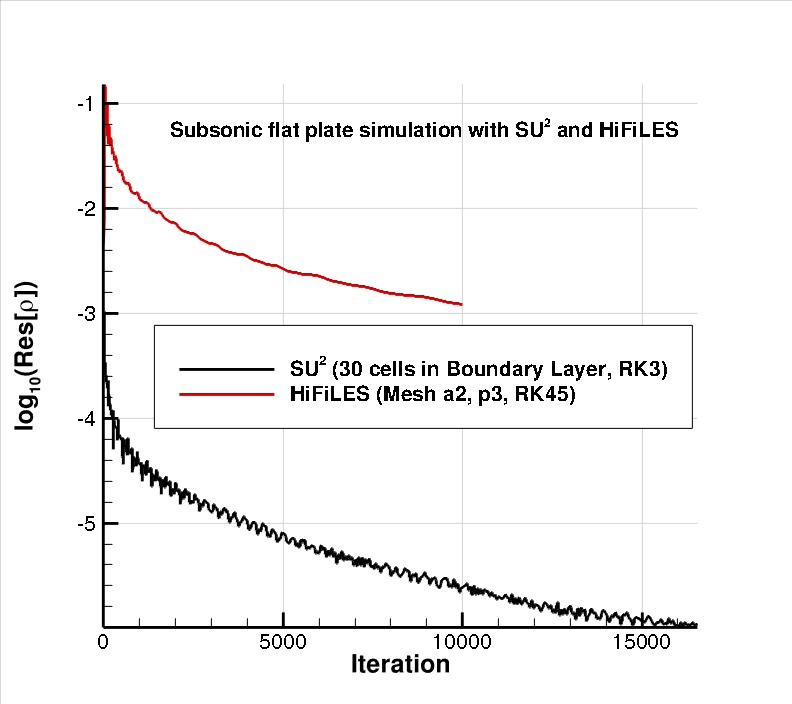
\includegraphics[width = \textwidth,clip=] {CompSu2.jpg}
\caption{Comparison of HiFiLES with SU$^2$ using a similar time integration scheme.}
\label{fig:Comparison_SecondOrder}
\end{minipage}
\end{center}
\end{figure}

To finalize, it is critical to note that the absence of a local time stepping technique in HiFiLES increases the required number of iterations to obtain a converged solution. However, we have noticed an improvement of the rate of converge as we refine the grid (see Fig. \ref{fig:ComparisonOrder}). Finally, the obtained convergence rate is comparable to a second order numerical code (e.g. SU$^2$\cite{palacios13,palacios14}) running using a similar numerical time integration (see Fig.\ref{fig:Comparison_SecondOrder}).


% Circular cylinder
% !TEX root = ./main.tex
\graphicspath{{figures_cylinder/}}% Set graphics path location

\subsection{Circular Cylinder}

The classic test case of laminar flow past a circular cylinder at low Reynolds number has also been chosen as a verification and validation case for the 2D Navier-Stokes equations in HiFiLES, and the results are compared to existing experimental data and simulation results~\cite{park1998}. Two separate cases are computed: first, the steady flow past the cylinder at $Re = 20$, and second, the unsteady flow past the cylinder at $Re = 100$, where the Reynolds number is based upon the diameter of the cylinder. For both cases, the Mach number is set to 0.1 in order to recover nearly incompressible flow for comparisons with the existing incompressible results. The remaining flow conditions are 0$\degr$ angle of attack, a constant ratio of specific heats of $1.4$, a Prandtl number of $0.72$, a free-stream temperature of 300 $K$, and a free-stream dynamic viscosity of $1.853\cdot 10^{-5} Pa \cdot s$ (laminar viscosity varies according to Sutherland's law during the simulation).

The two simulations are performed with third order polynomials on a mesh with 4988 total elements that contains quadrilateral elements near the body of the cylinder and triangular elements out to the far-field. There is a small refinement box immediately downstream of the cylinder to help resolve features in the wake. The rectangular far-field boundaries are located approximately 30 diameters away from the cylinder in the upstream, upward, and downward directions and 50 diameters away in the downstream direction. A view of the mesh near the cylinder surface is show in Fig.~\ref{cylinder_1}.

\begin{figure}
  \begin{subfigmatrix}{2}
    \subfigure[Zoom view of the mesh near the cylinder.]{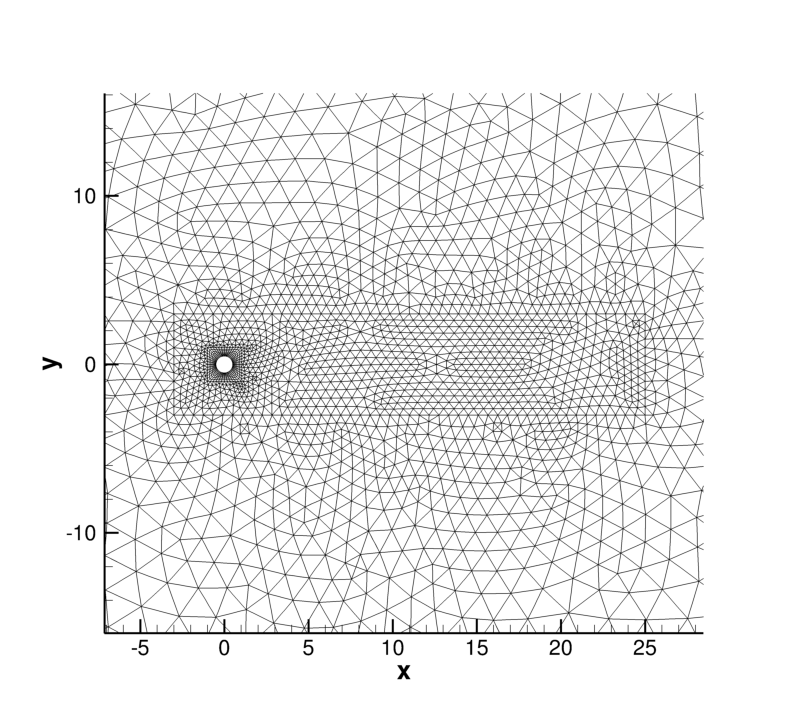
\includegraphics{cylinder_mesh.png}}
    \subfigure[X-velocity contours and streamlines around the circular cylinder for $Re = 20$.]{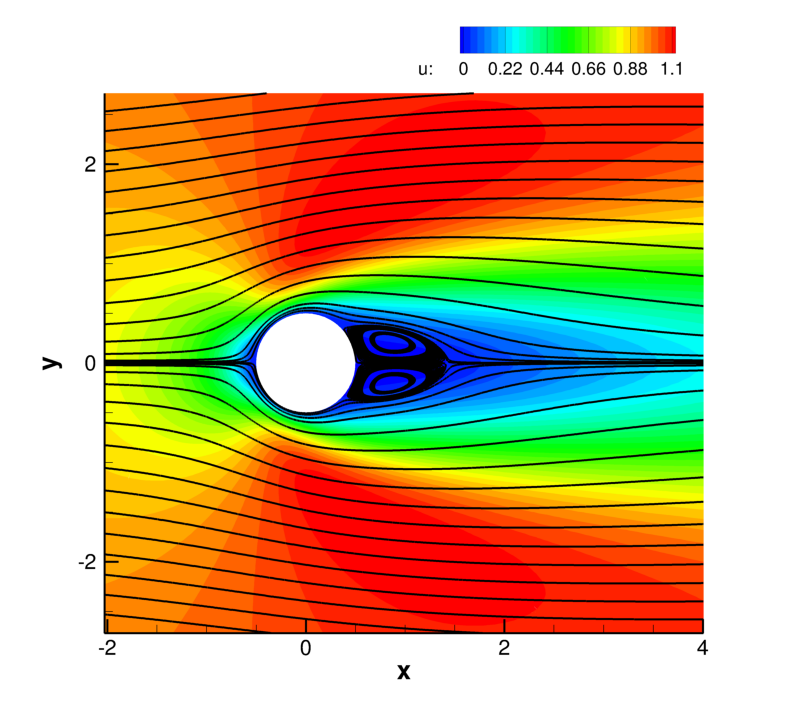
\includegraphics{cylinder_streamlines.png}}
  \end{subfigmatrix}
  \caption{The mesh for the circular cylinder simulations along with x-velocity contours for the $Re = 20$ case.}
  \label{cylinder_1}
\end{figure}

The flow around the cylinder for $Re = 20$ is steady, and it features a large recirculation region behind the cylinder. Fig.~\ref{cylinder_1} presents x-velocity contours around the cylinder along with streamlines. The length of the recirculation region can be determined from the streamlines, and a length of approximately one cylinder diameter agrees well with reported results for $Re = 20$. The coefficient of drag computed by HiFiLES is 2.043, which is close to the value of 2.01 reported by Park et al. Pressure contours around the cylinder are shown in Fig.~\ref{cylinder_2}.

\begin{figure}
  \begin{subfigmatrix}{2}
    \subfigure[Pressure contours for the $Re = 20$ case.]{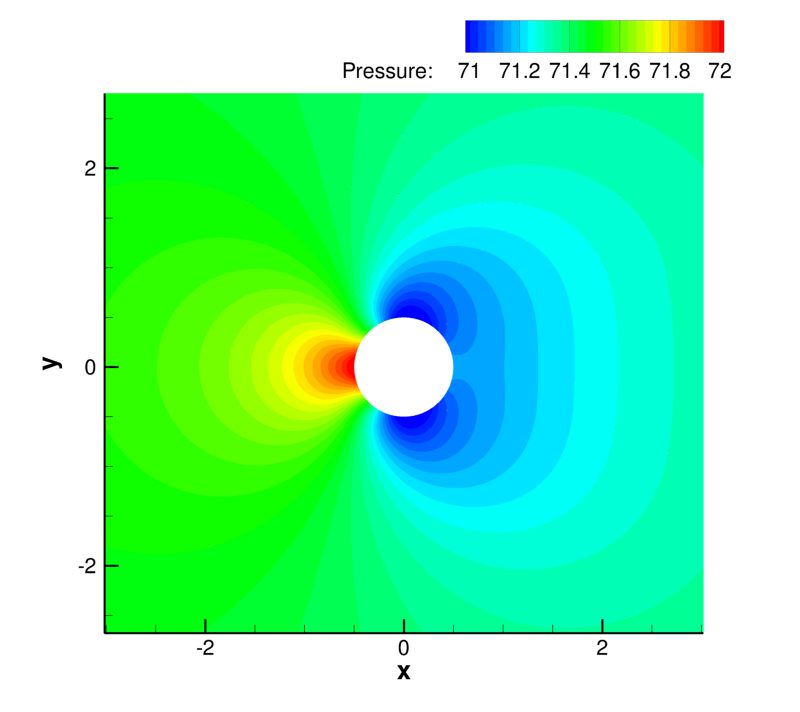
\includegraphics{cylinder_pressure_re20.png}}
    \subfigure[Pressure contours for the $Re = 100$ case.]{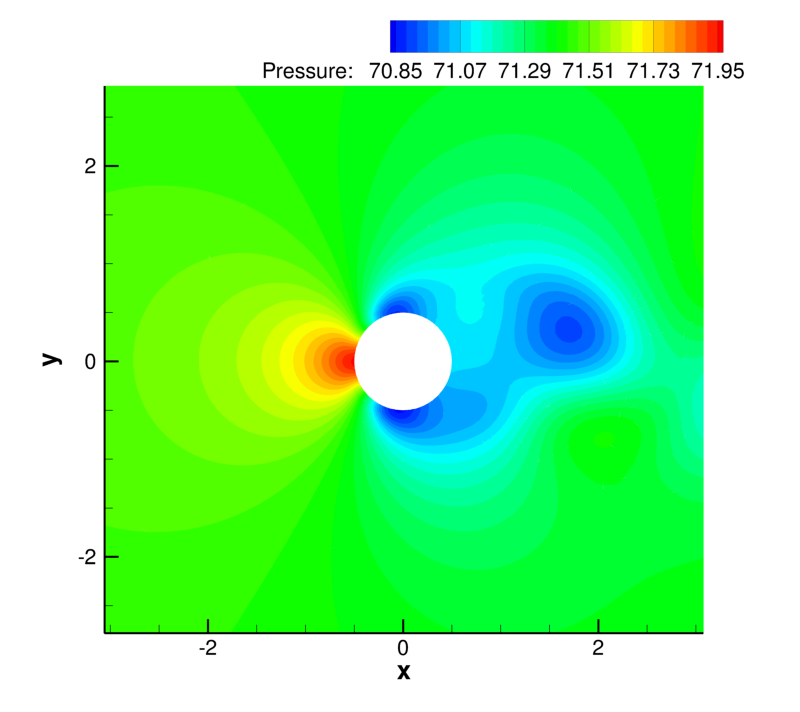
\includegraphics{cylinder_pressure_re100.png}}
  \end{subfigmatrix}
  \caption{Pressure contours for the steady and unsteady (instantaneous) cylinder cases.}
  \label{cylinder_2}
\end{figure}

When the Reynolds number is increased to 100, the flow around the cylinder becomes unsteady and exhibits periodic vortex shedding. This periodic shedding in the wake behind the cylinder can be seen in the instantaneous contours of x-velocity and vorticity in Fig.~\ref{cylinder_3}, and it also results in periodic fluctuations in the force coefficients on the cylinder. HiFiLES reports an average drag coefficient of 1.339 with a maximum deviation from this value of 0.0092, which agree excellently with the values reported by Park et al. of 1.33 and 0.0091 for the average $C_d$ and maximum deviation from it, respectively.  Instantaneous pressure contours for the $Re = 100$ case can be seen in Fig.~\ref{cylinder_2}. The asymmetry that is visible in the pressure contours contributes to the variability in the drag coefficient.

\begin{figure}
  \begin{subfigmatrix}{2}
    \subfigure[X-velocity contours around the circular cylinder for $Re = 100$.]{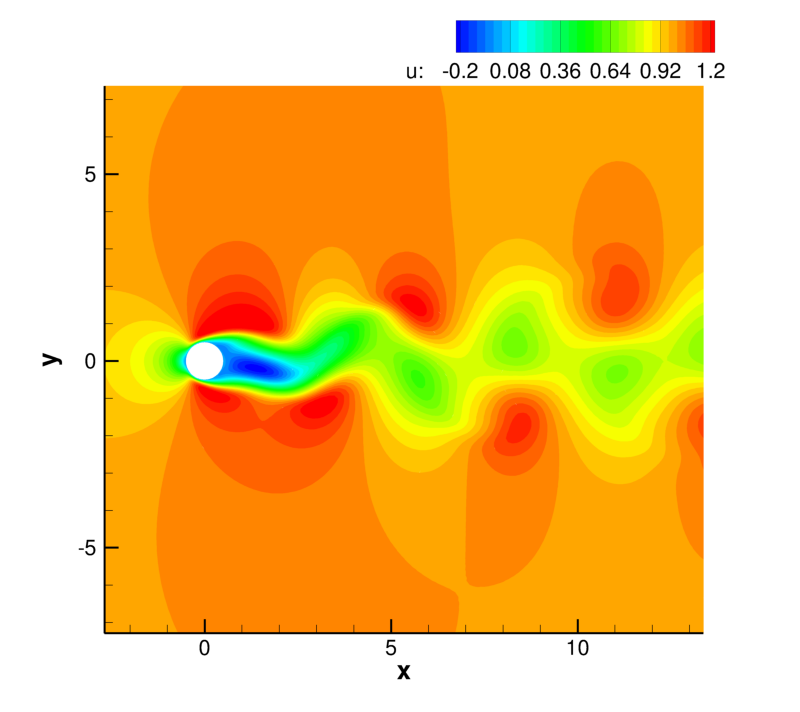
\includegraphics{cylinder_xvelocity_re100.png}}
    \subfigure[Vorticity contours for the $Re = 100$ case.]{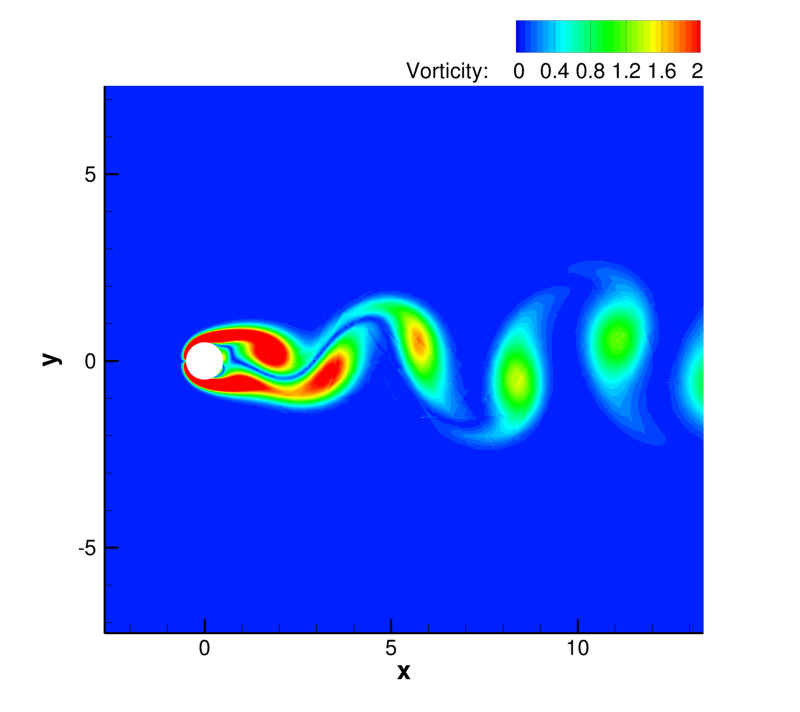
\includegraphics{cylinder_vorticity_re100.png}}
  \end{subfigmatrix}
  \caption{Instantaneous solution contours for the unsteady cylinder case.}
  \label{cylinder_3}
\end{figure}

% SD7003 section
% !TEX root = ./main.tex
\graphicspath{{figures_SD7003/}}% Set graphics path location

\subsection{SD7003 airfoil at 4$\degr$ angle of attack}\label{sd7003airfoil}

Abundant literature documents flow around a SD7003 infinite wing and airfoil. Hence, physical experiments \cite{ol2005comparison,radespiel2007numerical} and numerical simulations \cite{galbraith2008implicit,visbal2009high,castonguay2010simulation,persson2010high,uranga2011implicit} of flow over this geometry can be used to benchmark HiFiLES.

The simulations on the 2D geometry were performed on a circular domain with a radius of $50c$, where $c$ is the airfoil's cord length, centered at the leading edge of the airfoil. The boundary conditions are characteristic on the outer edge and adiabatic no-slip wall on the airfoil. The Mach number for all simulations was $M = 0.2$. The reported lift and drag coefficients in Table \eqref{table:sdAirfoilForce} correspond to the average of lift and drag coefficients over 13 periods after the flow reached a pseudo-periodic state. More details are provided by Williams\cite{williams2013thesis}. 

\begin{table}[htbp]
\centering
\begin{tabular}{ l| l l| l l| l l} 
  
 &  \multicolumn{2}{|c|}{$Re = 10K$}  & \multicolumn{2}{|c|}{$Re = 22K$} & \multicolumn{2}{|c}{$Re = 22K$}  \\ 
 Source & $C_L$ & $C_D$ & $C_L$ & $C_D$ & $C_L$ & $C_D$   \\ 
\hline
 Uranga et al.\cite{uranga2011implicit} & 0.3755 & 0.04978 & 0.6707 & 0.04510 & 0.5730 & 0.02097  \\ 
$c_{dg},\kappa_{dg}$ & 0.3719 & 0.04940 & 0.6722 & 0.04295 & 0.5831 & 0.01975 \\ 
$c_{+},\kappa_{+}$ & 0.3713 & 0.04935 & 0.6655 & 0.04275 & 0.5774 & 0.02005  \\ 
 \end{tabular}
\caption{Time-averaged values of the lift and drag coefficients for the SD7003 airfoil flows with $Re = 10,000, 22,000, 60,000$}
\label{table:sdAirfoilForce} 
 \end{table}

\begin{figure}[htbp]
\centering
\subfigure[Density contours]{
\includegraphics*[trim=0 0 0 0,width=0.48\textwidth]{figure_935a}}
\subfigure[Vorticity contours]{
\includegraphics*[trim=0 0 0 0,width=0.48\textwidth]{figure_935b}}\\

\caption{Density and vorticity contours for the flow with $Re = 10,000$ around the SD7003 airfoil. $p=2$ on unstructured triangular grid with $N = 25,810$ elements}
\label{sdairfoilre10k}
\end{figure}

\begin{figure}[htbp]
\centering
\subfigure[Density contours]{
\includegraphics*[trim=0 0 0 0,width=0.48\textwidth]{figure_936a}}
\subfigure[Vorticity contours]{
\includegraphics*[trim=0 0 0 0,width=0.48\textwidth]{figure_936b}}\\

\caption{Density and vorticity contours for the flow with $Re = 22,000$ around the SD7003 airfoil. $p=2$ on unstructured triangular grid with $N = 25,810$ elements}
\label{sdairfoilre22k}
\end{figure}

\begin{figure}[htbp]
\centering
\subfigure[Density contours]{
\includegraphics*[trim=0 0 0 0,width=0.48\textwidth]{figure_937a}}
\subfigure[Vorticity contours]{
\includegraphics*[trim=0 0 0 0,width=0.48\textwidth]{figure_937b}}\\

\caption{Density and vorticity contours for the flow with $Re = 60,000$ around the SD7003 airfoil. $p=2$ on unstructured triangular grid with $N = 25,810$ elements}
\label{sdairfoilre60k}
\end{figure}

The average lift and drag coefficients are in close agreement with the results by Uranga el. al\cite{uranga2011implicit}. The density contours in Figures \eqref{sdairfoilre10k},\eqref{sdairfoilre22k}, and \eqref{sdairfoilre60k} show that vortical structures are captured for a reasonable distance away from the airfoil despite the fact that elements are coarser away from the airfoil.


\newpage

\subsection{SD7003 wing section at 4$\degr$ angle of attack}
To validate HiFiLES's performance in 3D simulations, we extrude the SD7003 geometry from Section\eqref{sd7003airfoil} by $0.2c$ in the $z$-direction and apply periodic boundary conditions at $z=0$ and $z=0.2c$. Table \eqref{table:sdWingForce} shows the time-averaged lift and drag coefficients.


\begin{table}[htbp]
\centering
\begin{tabular}{ l| l l| l l| l l} 
  
 &  \multicolumn{2}{|c|}{$Re = 10K$}  \\ 
 Source & $C_L$ & $C_D$    \\ 
\hline
 Uranga et al.\cite{uranga2011implicit} & 0.3743 & 0.04967   \\ 
$c_{dg},\kappa_{dg}$ & 0.3466 & 0.04908  \\ 
$c_{+},\kappa_{+}$ & 0.3454 & 0.04903 \\ 
 \end{tabular}
\caption{Time-averaged values of the lift and drag coefficients for the SD7003 wing-section in a flow with $Re = 10,000$}
\label{table:sdWingForce} 
 \end{table}


\begin{figure}[htbp]
\centering
\subfigure[Density contours]{
\includegraphics*[trim=0 0 0 0,width=0.48\textwidth]{figure_939a}}
\subfigure[Vorticity contours]{
\includegraphics*[trim=0 0 0 0,width=0.48\textwidth]{figure_939b}}\\

\caption{Density and vorticity isosurfaces colored by Mach number for the flow with $Re = 10,000$ around the SD7003 wing-section. $p=3$ on unstructured tetrahedral grid with $N = 711,332$ elements}
\label{sdwingre10k}
\end{figure}

It is worth noting that the vortical structures are preserved better than in the 2D case. Table \eqref{table:sdWingForce} demonstrates that HiFiLES provides average lift and drag coefficient estimates in close agreement with experiments.



% Taylor-Green Vortex
% !TEX root = ./main.tex
\graphicspath{{figures_taylorgreen/}}% Set graphics path location

\subsection{Taylor-Green Vortex at Re = 1,600}

The Taylor-Green Vortex (TGV) is a simple test of the resolution of the small scales of a turbulent flow by a numerical method.
The compressible TGV at $Re=1600$ was one of the benchmark problems in the 1st and 2nd International Workshops on High-Order CFD Methods~\cite{wang2013}.
A reference solution was computed by Debonis~\cite{debonis:13} using a high-order dispersion relation-preserving (DRP) scheme on a mesh of $512^3$ elements.
The results presented here were obtained by Bull and Jameson using FR to recover the fourth-order-accurate DG and SD schemes in HiFiLES~\cite{bull2014a,bull2014b}.
We also compare our results to those of Beck and Gassner~\cite{beck:12}, who used a fourth-order filtered DG method on a mesh of $64^3$ elements.
From a simple initial condition in a triply-periodic box of dimensions $[0:2\pi]^3$, interactions between vortices cause the flow to develop in a prescribed manner into a mass of elongated vortices across a range of scales.
The initial condition is specified as
%
\begin{eqnarray}\label{tgv}
u(t_0) &&= u_0 \sin (x/L) \cos (y/L) \cos (z/L), \\
v(t_0) &&= -u_0 \cos (x/L) \sin (y/L) \cos (z/L), \\
w(t_0) &&= 0, \\
p(t_0) &&= p_0 + \frac{\rho_0 V^2_0}{16} \left [ \cos \left (\frac{2x}{L} \right ) + \cos \left (\frac{2y}{L} \right ) \right ] \left [ \cos \left (\frac{2z}{L} \right ) + 2 \right ],
\end{eqnarray}
%
where $L = 1$, $u_0 = 1$, $\rho_0 = 1$ and $p_0 = 100$.
The Mach number is set to 0.08 (consistent with the initial pressure $p_0$) and the initial temperature is 300K.

Figs.~\ref{dissrate} (a) and (b) show the volume-averaged kinetic energy $\langle k \rangle$  on (a) hexahedral meshes of $16^3$, $32^3$ and $64^3$ elements and (b) tetrahedral meshes (formed by splitting the hexahedral meshes in six).
The reference solution, labelled as`DRP-512' is plotted for comparison.
Figs.~\ref{dissrate} (c) and (d) show the kinetic energy dissipation rate, given by $\epsilon = -d \langle k \rangle/dt$ versus the reference solution and the results of Beck and Gassner~\cite{beck:12}, labelled as`Beck-DG-64x4'.
On the finest hexahedral and tetrahedral meshes the kinetic energy and dissipation rate predictions match the reference solution, demonstrating that the high-order numerical scheme is able to resolve the important flow dynamics on a relatively coarse mesh.
As a qualitative measure of the resolution of the turbulent flow structures, Figure \ref{qcrit} shows isosurfaces of the $q$ criterion at four times during the simulation.
The evolution of complex small scale structures is evident.

\begin{figure}[htbp]
\centering
\subfigure[$\langle k \rangle$, hexahedral meshes]{
\includegraphics*[trim=0 0 0 0,width=0.48\textwidth]{tke-SD-hex-mesh}}
\subfigure[$\langle k \rangle$, tetrahedral meshes]{
\includegraphics*[trim=0 0 0 0,width=0.48\textwidth]{tke-SD-tet-mesh.pdf}}\\
\subfigure[$-d \langle k \rangle/dt$, hexahedral meshes]{
\includegraphics*[trim=0 0 0 0,width=0.48\textwidth]{dissrate-SD-hex-mesh.pdf}}
\subfigure[$-d \langle k \rangle/dt$, tetrahedral meshes]{
\includegraphics*[trim=0 0 0 0,width=0.48\textwidth]{dissrate-SD-tet-mesh.pdf}}\\
\caption{\small Taylor-Green vortex results on hexahedral and tetrahedral meshes from Bull and Jameson~\cite{bull2014a}.
(a, b) Evolution of average kinetic energy $\langle k \rangle$; (c, d) dissipation rate $-d \langle k \rangle/dt$.
`SD-$M \times N$' refers to $M^3$ mesh, $N$th-order accurate SD scheme.
(\textbf{- - -}) 4th-order DG on $64^3$ mesh~\cite{beck:12}; ($\circ$) DNS~\cite{debonis:13}.}
\label{dissrate}
\end{figure}

\begin{figure}[htbp]
\centering
\subfigure[$t = 2.5$, $Q=0.5$]{
\includegraphics*[width=0.48\textwidth]{TGV-DG3-hex-64-qcriterion-isosurface-005-velocolor-025s-z-small}}
\subfigure[$t = 5$, $Q=1.5$]{
\includegraphics*[width=0.48\textwidth]{TGV-DG3-hex-64-qcriterion-isosurface-015-velocolor-05s-z-small}}\\
\subfigure[$t = 7.5$, $Q=1.5$]{
\includegraphics*[width=0.48\textwidth]{TGV-DG3-hex-64-qcriterion-isosurface-015-velocolor-075s-z-small}}
\subfigure[$t = 10.75$, $Q=1.5$]{
\includegraphics*[width=0.48\textwidth]{TGV-DG3-hex-64-qcriterion-isosurface-015-velocolor-1075s-z-small}}
\caption{TGV solution on the fine mesh using fourth order accurate DG method, showing isosurfaces of $q$ criterion colored by velocity magnitude at time $t$ = 2.5 to 10.75 seconds.}
\label{qcrit}
\end{figure}



%Square Cylinder
% !TEX root = ./main.tex
\graphicspath{{figures_squarecylinder/}}% Set graphics path location

\subsection{LES of Flow Over a Square Cylinder at Re = 21,400}\label{sqcyl}

Using the FR method to recover the fourth-order accurate SD scheme, the flow over a square cylinder of side $D$ in a domain of $21D \times 12D \times 3.2D$ (see Figure \ref{sqcylmesh}) at $Re = 21,400$ and Mach 0.3 was simulated, for which LDV experimental data is available~\cite{lyn1994,lyn1995}.
A tetrahedral mesh of 87,178 elements was generated giving a total of 1.74M degrees of freedom (D0F) since there are 20 solution points per element at fourth order accuracy.
Time discretization was by the fourth-order five-stage explicit RK scheme.
A total time of 250 seconds was simulated and time-averaged quantities were calculated over the last 100 seconds (approx. 5 flow-through periods).
The WSM model (see Section \ref{lesmodels}) based on the modal Vandermonde filter~\cite{bull2013a} was used with the Breuer-Rodi three-layer wall model~\cite{breuer1994} within 0.2D of the wall.
The computation took around 60 hours on 7 GPUs in the lab's own cluster.
Figure \ref{sqcylmesh} shows the computational mesh including all the DoF.
Figure \ref{sqcylqcrit} shows an isosurface of the $q$-criterion colored by velocity magnitude, illustrating the structures present in the turbulent boundary layer and wake.
Figures \ref{sqcylplots} (a, b) show the normalized mean streamwise and vertical velocity components $\langle u \rangle/u_B$ and $\langle v \rangle/u_B$ respectively along several vertical lines in the wake.
Figures \ref{sqcylplots} (c, d) show the normalized mean Reynolds stress components $\langle u'u' \rangle/u_B^2$ and $\langle u'v' \rangle/u_B^2$ along the same lines.
For comparison, high-order LES results computed by by Lodato and Jameson~\cite{lodato2012b} using the SD method and the WSM model on a hexahedral mesh of 2.3M DoF are plotted.
Mean velocities are accurately predicted although the accuracy is reduced near the cylinder owing to the coarse tetrahedral resolution in the boundary layer.
The Reynolds stresses are less accurately predicted than the mean velocities but are broadly correct.
These results highlight the advantages of using HiFiLES for LES of turbulent flows: the ability to obtain good results on coarse meshes and the ability to use unstructured tetrahedral meshes.


\begin{figure}[h] \tt
\centering
\subfigure[geometry]{
\includegraphics*[width=0.61\textwidth]{sqcyl-geom-small}}
\subfigure[boundary layer mesh]{
\includegraphics*[width=0.35\textwidth]{sqcyl-tet-coarse3-blmesh}}
\caption{Square cylinder geometry and tetrahedral boundary layer mesh showing all degrees of freedom}
\label{sqcylmesh}
\end{figure}

\begin{figure}[h] \tt
\centering
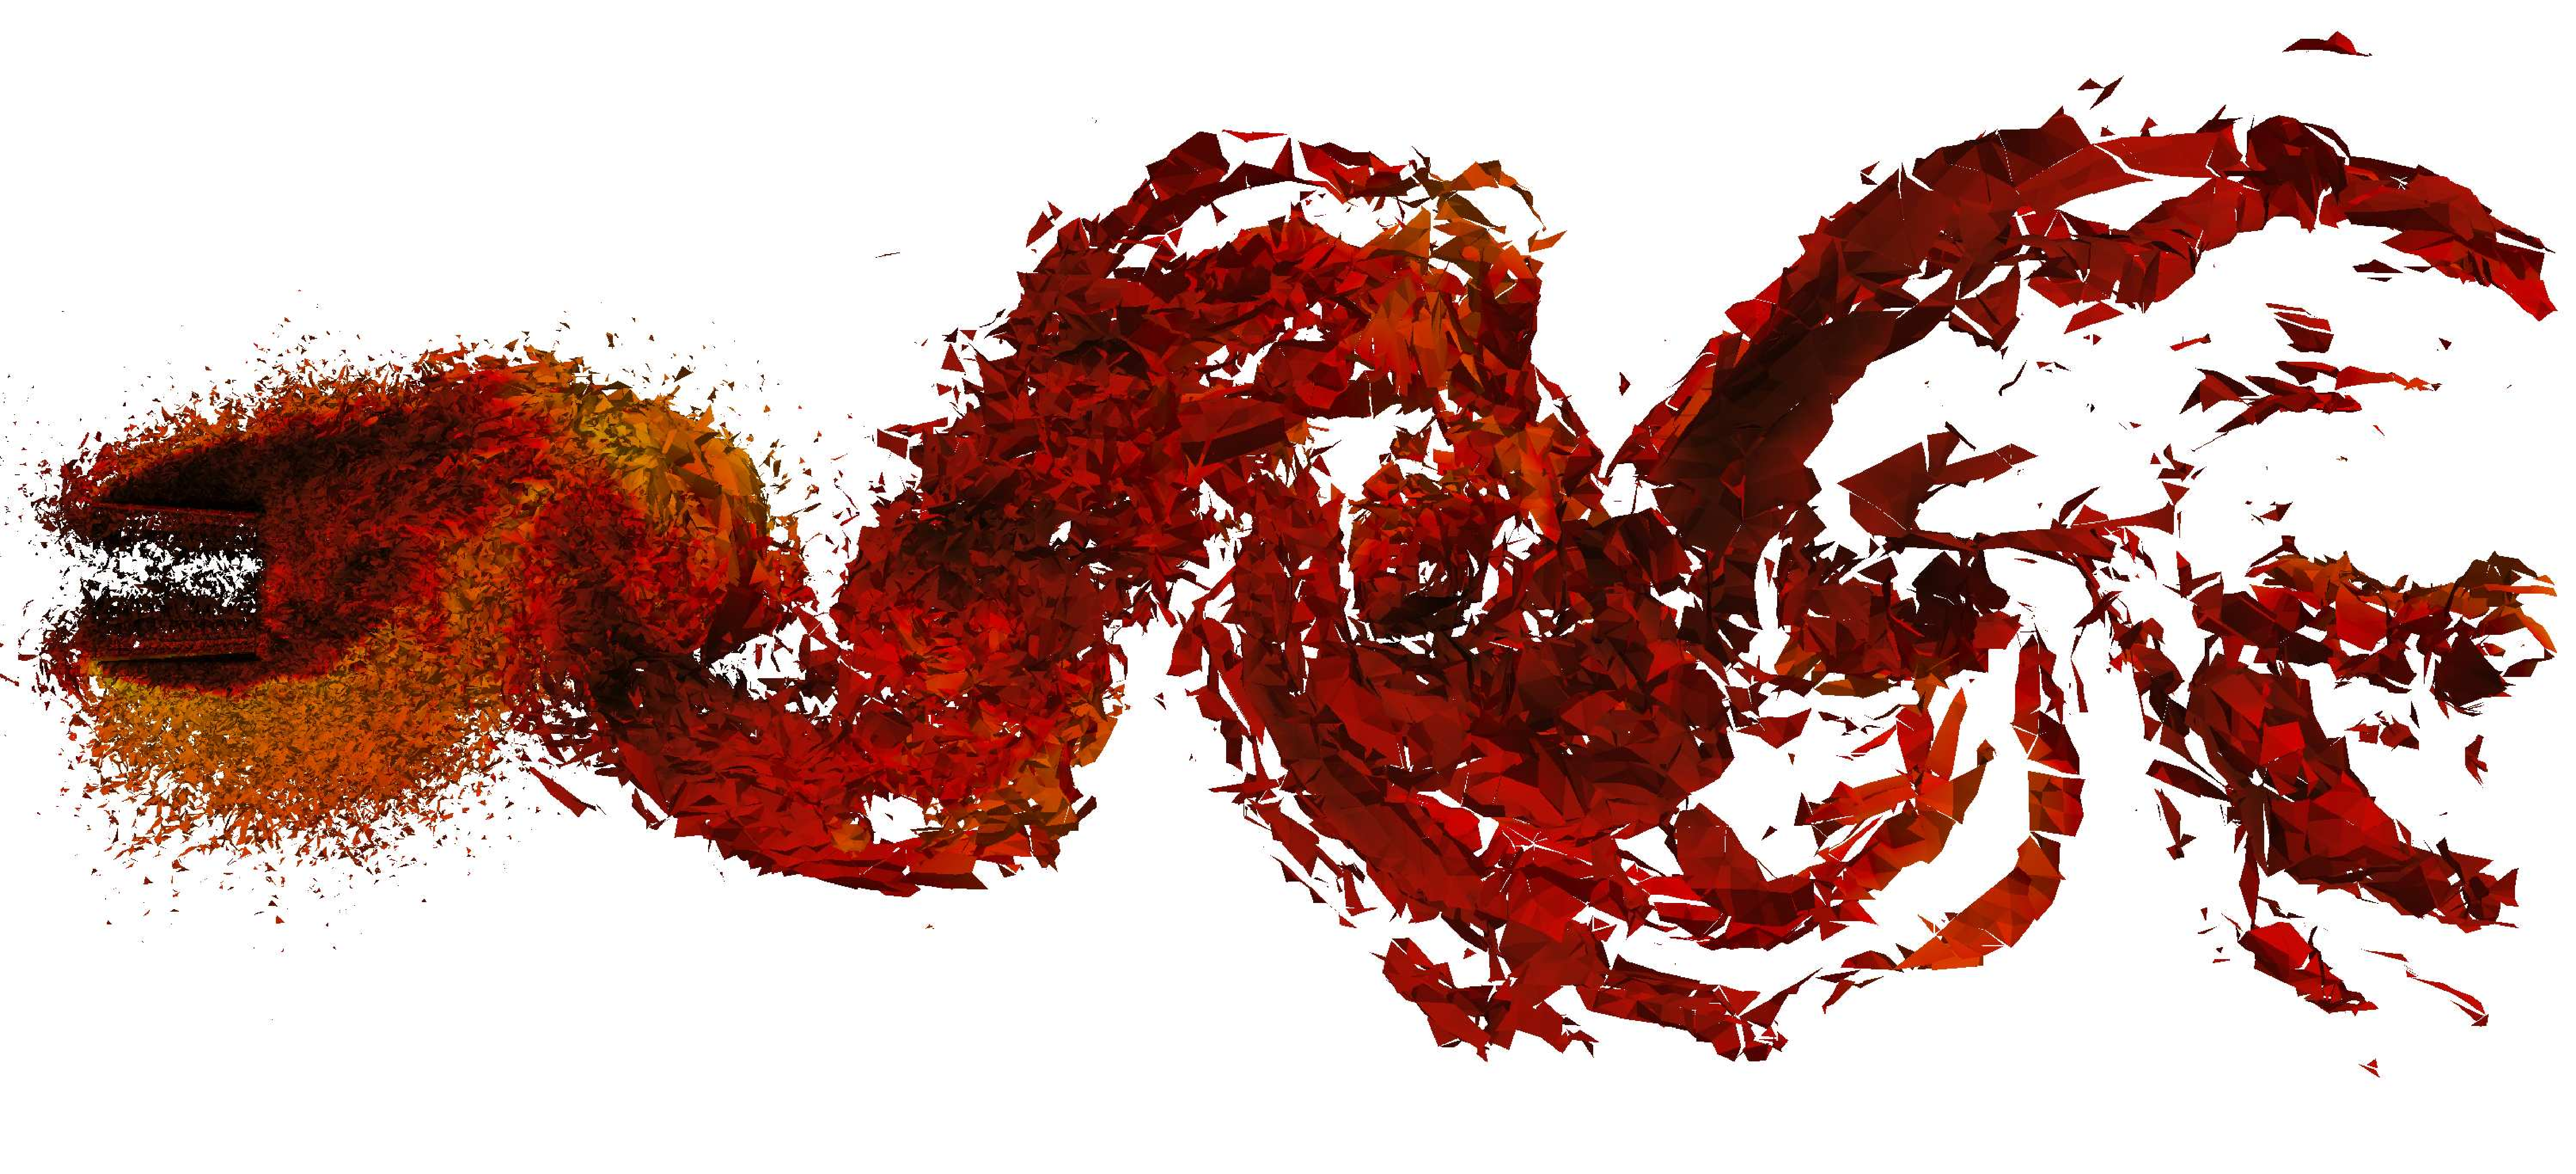
\includegraphics[width=0.9\textwidth]{sqcyl-tet-wsm-newwallfn-coarse3-qcrit-010-velomag.pdf}
\caption{Isosurface of the $q$-criterion colored by velocity magnitude showing the wake behind the square cylinder}
\label{sqcylqcrit}
\end{figure}

\begin{figure}[h]
\centering
\subfigure[Mean streamwise velocity $\langle u \rangle/u_B$]{
\includegraphics*[width=0.8\textwidth]{sqcyl-tet-wsm-newfilt-coarse-fixbc-meanu-vprofile-small.pdf}}\\
\subfigure[Mean vertical velocity $\langle v \rangle/u_B$]{
\includegraphics*[width=0.8\textwidth]{sqcyl-tet-wsm-newfilt-coarse-fixbc-meanv-vprofile-small.pdf}}\\
\subfigure[Mean Reynolds stress $\langle u'u' \rangle/u_B^2$]{
\includegraphics*[width=0.8\textwidth]{sqcyl-tet-wsm-newfilt-coarse-fixbc-meanuu-vprofile-small.pdf}}\\
\subfigure[Mean Reynolds stress $\langle u'v' \rangle/u_B^2$]{
\includegraphics*[width=0.8\textwidth]{sqcyl-tet-wsm-newfilt-coarse-fixbc-meanuv-vprofile-small.pdf}}
\caption{\small (a) Mean streamwise and vertical velocity and mean Reynolds stresses along vertical lines in the wake.
(---) current results, (- - - ) 4th order SD+WSM on hexahedral mesh by Lodato and Jameson~\cite{lodato2012b}, ($\circ$) LDV experiments by Lyn et al.~\cite{lyn1994,lyn1995}.}
\label{sqcylplots}
\end{figure}



